%%%%%%
%
% $Author: Abishek $
% $Date: 06.05.2024 $
% $Path: BA24-02-Time-Series\report\Contents\en$
% $Version: 1.0 $
%
%
% !TeX encoding = utf8
% !TeX root = Rename
% !TeX TXS-program:bibliography = txs:///bibtex
\section{Test Complete System}

The entire system was tested rigorously to ensure it performs as expected for all functional and operational requirements. The testing process covered both hardware and software components, focusing on integration, performance, and reliability.

\subsection{Test System's Functions}
The system was tested to confirm that it correctly captures IMU data, processes it, and classifies gait patterns as normal or Parkinsonian. The RGB output on the Arduino Nano BLE Sense was observed to confirm the classification result:
\begin{itemize}
	\item \textbf{Normal Gait}: Red LED lights up\ref{fig:Output Display}.
	\item \textbf{Parkinsonian Gait}: Blue LED lights up.
\end{itemize}

\begin{figure}[h]
	\centering
	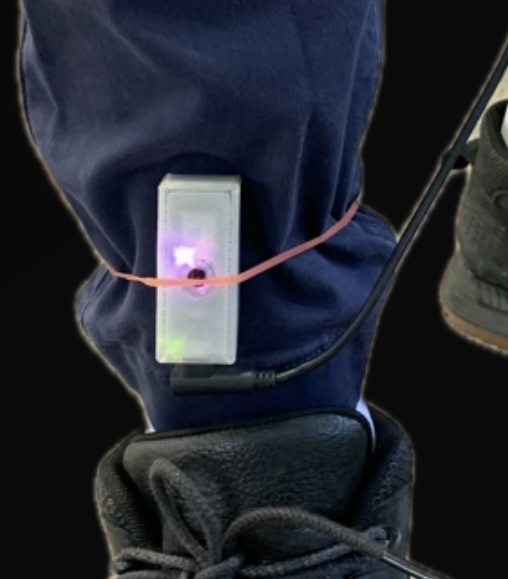
\includegraphics[width=0.7\textwidth]{Images/prototypeR}
	\caption{Output Display}
	\label{fig:Output Display}
\end{figure}

Tests ensured that the system’s functions were consistent and error-free across multiple trials and environmental conditions.

\subsection{Test Parts}
Each component of the system was individually tested to verify its functionality:
\begin{itemize}
	
	\item \textbf{Power Management}: The Arduino board was monitored to ensure it could handle continuous operation without overheating or power failure.
	\item \textbf{Hardware Components}: The accuracy of the IMU (Inertial Measurement Unit) sensor was rigorously tested to ensure suitability for gait analysis. During static testing, the IMU was placed on a stable, motionless surface to evaluate its precision. The accelerometer readings were verified to measure approximately 9.8 m/s² along the axis aligned with gravity, while the other axes displayed near-zero values. The gyroscope was assessed to ensure it produced zero angular velocity (0 rad/s) across all axes when stationary. Additionally, the magnetometer readings were compared against the Earth’s magnetic field strength specific to the test location, ensuring accurate sensor calibration.\cite{Zujevs2019IMUCalibration}
\end{itemize}

\subsection{Test Software Modules}
The software pipeline was divided into modules, and each module was tested independently:
\begin{itemize}
	\item \textbf{Data Preprocessing Module}: The \texttt{kalmanfilter.py} was tested using noisy IMU data to ensure it effectively smoothed out noise without losing essential gait features.
	\item \textbf{Model Training Module}: The CNN model was trained and evaluated on test data, ensuring high accuracy in classifying normal and Parkinsonian gaits.
	\item \textbf{Export Module}: The \texttt{tfliteexporter.py} was tested to confirm the TensorFlow Lite model was converted correctly into a \texttt{.h} file for Arduino integration.
\end{itemize}

\subsection{Test Software Classes}
For object-oriented components:
\begin{itemize}
	\item \textbf{DataLoader Class}: Tested for proper loading and handling of \texttt{normalpatterns.csv} and \texttt{parkinsonpatterns.csv} datasets, ensuring missing or corrupted data was handled gracefully.
	\item \textbf{Visualization Class}: Verified it generated accurate and interpretable plots of model performance (e.g., accuracy, loss).\ref{fig:output}
\end{itemize}

\subsection{Test Software Functions}
Key functions within the modules were tested to ensure they returned the expected outputs:
\begin{itemize}
	\item \textbf{Feature Extraction Functions}: These were tested using sample gait data to confirm correct calculation of step length, stride time, and stride velocity.
	\item \textbf{Prediction Functions}: The CNN model’s prediction function was tested with preprocessed data to confirm correct classification labels (0 for normal, 1 for Parkinsonian).
\end{itemize}

\subsection{Automation of the Tests}
To ensure efficient and repeatable testing, automated scripts were developed using Python:
\begin{itemize}
	\item \textbf{Unit Tests}: Automated tests were written for each module using \texttt{unittest} to verify expected behavior.
	\item \textbf{End-to-End Testing}: Scripts simulated the entire pipeline, from data loading to BLE-based output verification, ensuring the system worked seamlessly.
\end{itemize}

\subsection{Test Protocol}
The testing protocol included the following steps:

\begin{figure}[h]
	\centering
	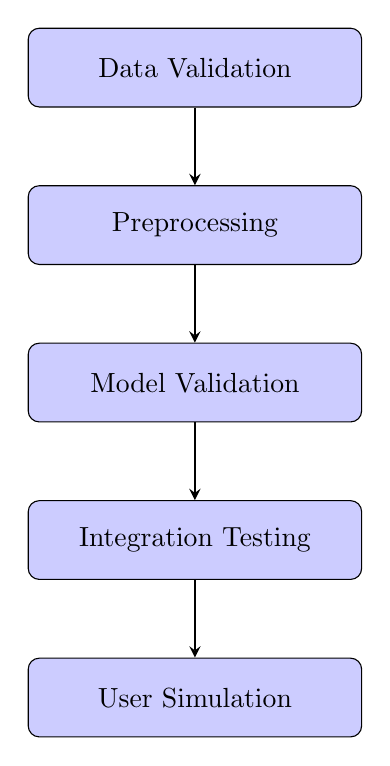
\begin{tikzpicture}[node distance=2.0cm, auto, align=center]
		% Node styles
		\tikzstyle{process} = [rectangle, draw, fill=blue!20, text width=4cm, minimum height=1cm, rounded corners]
		\tikzstyle{arrow} = [thick,->,>=stealth]
		
		% Nodes
		\node[process] (dataValidation) {Data Validation};
		\node[process, below of=dataValidation] (preprocessingValidation) {Preprocessing};
		\node[process, below of=preprocessingValidation] (modelValidation) {Model Validation};
		\node[process, below of=modelValidation] (integrationTesting) {Integration Testing};
		\node[process, below of=integrationTesting] (userSimulation) {User Simulation};
		
		% Arrows
		\draw[arrow] (dataValidation) -- (preprocessingValidation);
		\draw[arrow] (preprocessingValidation) -- (modelValidation);
		\draw[arrow] (modelValidation) -- (integrationTesting);
		\draw[arrow] (integrationTesting) -- (userSimulation);
	\end{tikzpicture}
	\caption{Key Validation Steps for the System}
	\label{fig:key_validation_steps}
\end{figure}

\begin{enumerate}
	\item \textbf{Data Validation}: Verified the integrity of input datasets.
	\item \textbf{Preprocessing Validation}: Checked if the Kalman filter smoothed data effectively.
	\item \textbf{Model Validation}: Evaluated the CNN model on a validation set, ensuring performance metrics (accuracy, precision, recall) met expected standards.
	\item \textbf{Integration Testing}: Confirmed that the pipeline integrated seamlessly with the Arduino device for real-time inference.
	\item \textbf{User Simulation}: Tested the system under real-world conditions by simulating normal and Parkinsonian gait patterns, observing the output on the Arduino’s RGB LED.
\end{enumerate}
